%   ------------------------------------------------------------------------
\FloatBarrier
\section{Análise do Vidu}
\label{s.vidu}

A ferramenta vidu foi escolhida por sua capacidade de gerar vídeos a partir de imagens. A funcionalidade que foi mais chamativa foi a geração de vídeos através de referências, que prometia manter a consistência dos personagens, lugares e objetos. Além dessa, o site também oferecia a geração de vídeo através de uma imagem, permitindo definir o frame inicial e final.No OpenArt.AI (descrito na Seção \ref{s.openArt}), era utilizado um dos modelos que pertence a essa ferramenta, o Vidu Q1, que é o modelo mais avançado do Vidu para a geração de vídeos, não disponível na plataforma para uso gratuito. Dessa forma, o modelo Vidu 2.0 foi o utilizado durante os testes.

%%% pablo, pablo lateral de alguma IA, ver tudo que pegou de fora
\begin{figure}[htbp]
    \centering
    \caption{\small Artefatos usados para referência no vidu}
    \label{fig:viduArtefatos}
    \begin{subfigure}{0.22\linewidth}
        
\includegraphics[width=0.7\linewidth]{figs/sprites/Pablo.PNG}
        \caption{\small Sprite do personagem Pablo em front view}
        \label{fig:viduPablo}
    \end{subfigure}
    \begin{subfigure}{0.22\linewidth}
        \centering
        
\includegraphics[width=1\linewidth]{figs/chatGPT/visao_lateral/res1.png}
        \caption{\small Sprite do personagem Pablo em side view gerado pelo ChatGPT}
        \label{fig:viduPabloChatGPTSide}
    \end{subfigure}
    \begin{subfigure}{0.22\linewidth}
        \centering
        
\includegraphics[width=1\linewidth]{figs/sprites/Pablo_sideView.png}
        \caption{\small Sprite do personagem Pablo em side view gerado pelo GeminiPro e editado no Pixel Lab}
        \label{fig:viduPabloGeminiProSide}
    \end{subfigure}
    \begin{subfigure}{0.22\linewidth}
        \centering
        
\includegraphics[width=1\linewidth]{figs/sprites/Pablo_backView.png}
        \caption{\small Sprite do personagem Pablo em back view (visão traseira, em inglês) gerado pelo GeminiPro e editado no Pixel Lab}
        \label{fig:viduPabloGeminiProBack}
    \end{subfigure}
    \begin{subfigure}{0.32\linewidth}
        \centering
        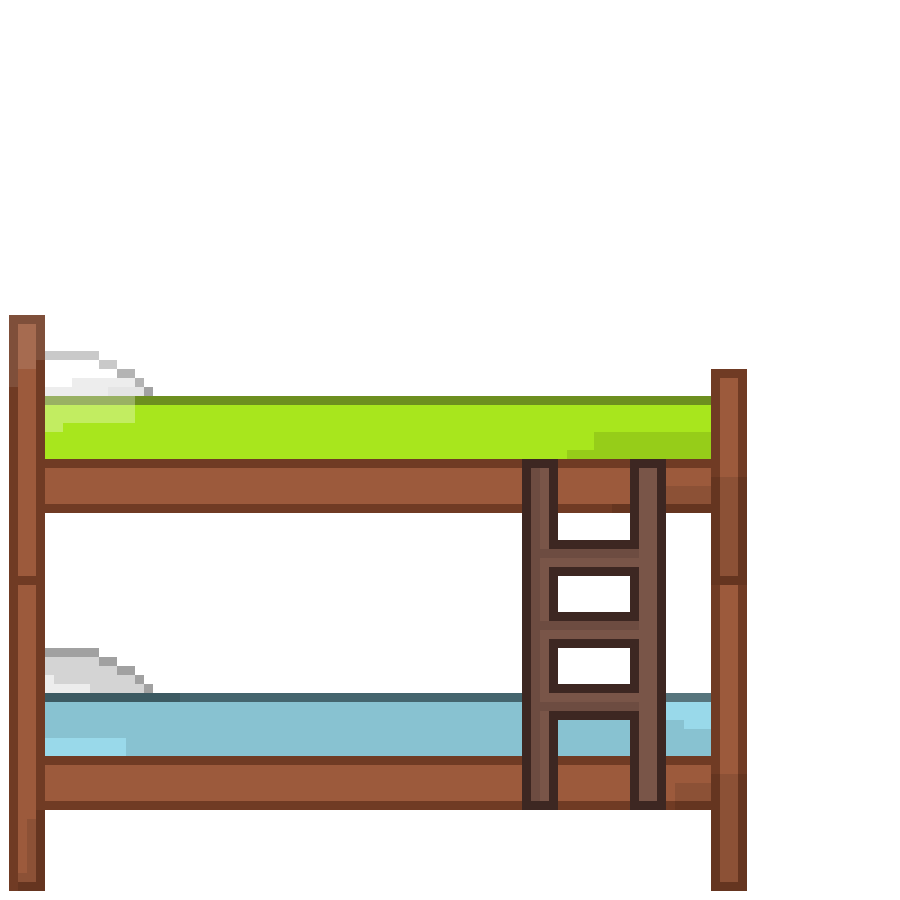
\includegraphics[width=1\linewidth]{figs/vidu/referencia_cama.png}
        \caption{\small Sprite da cama}
        \label{fig:viduCama}
    \end{subfigure}
    \begin{subfigure}{0.18\linewidth}
        \centering
        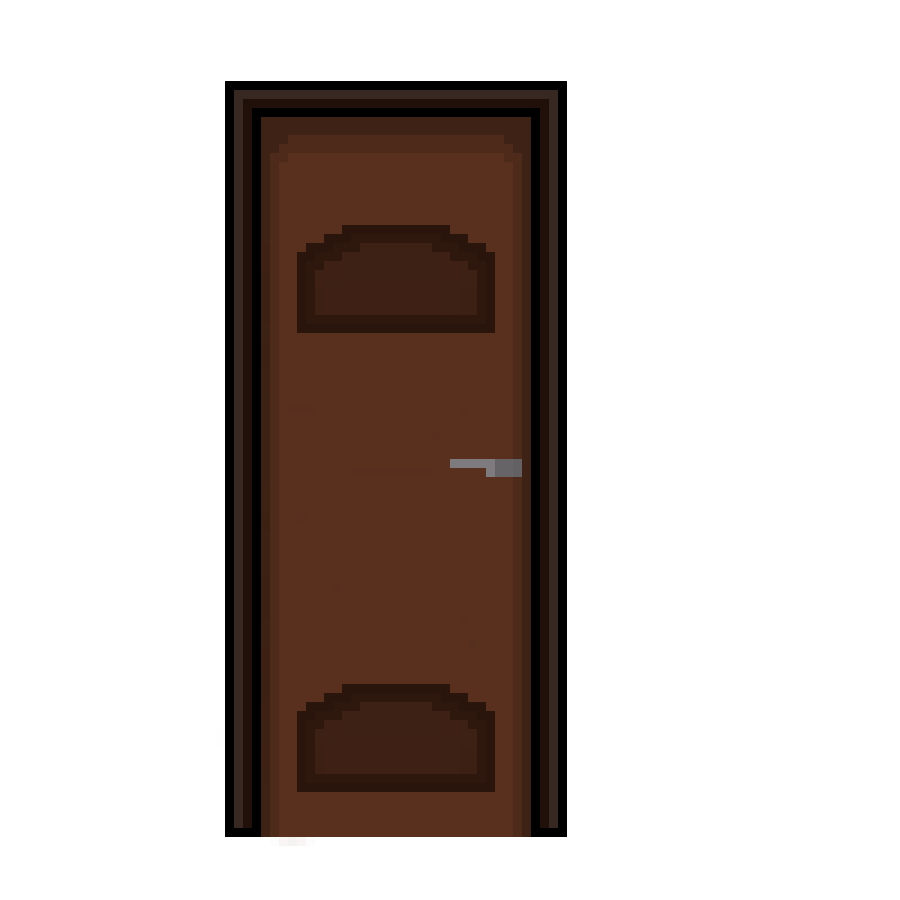
\includegraphics[width=1\linewidth]{figs/vidu/referencia_porta (1).png}
        \caption{\small Sprite da porta em front view}
        \label{fig:viduPortaA}
    \end{subfigure}
    \begin{subfigure}{0.18\linewidth}
        \centering
        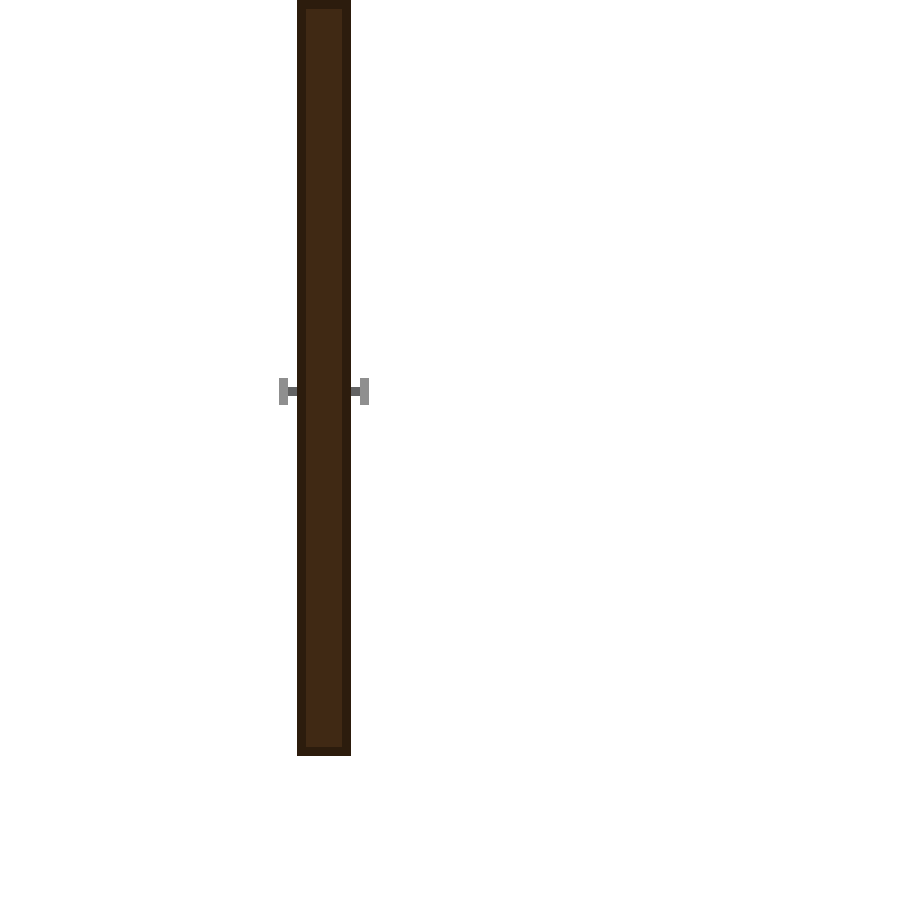
\includegraphics[width=1\linewidth]{figs/vidu/referencia_porta (2).png}
        \caption{\small Sprite da porta em side view}
        \label{fig:viduPortaB}
    \end{subfigure}
    \begin{subfigure}{0.18\linewidth}
        \centering
        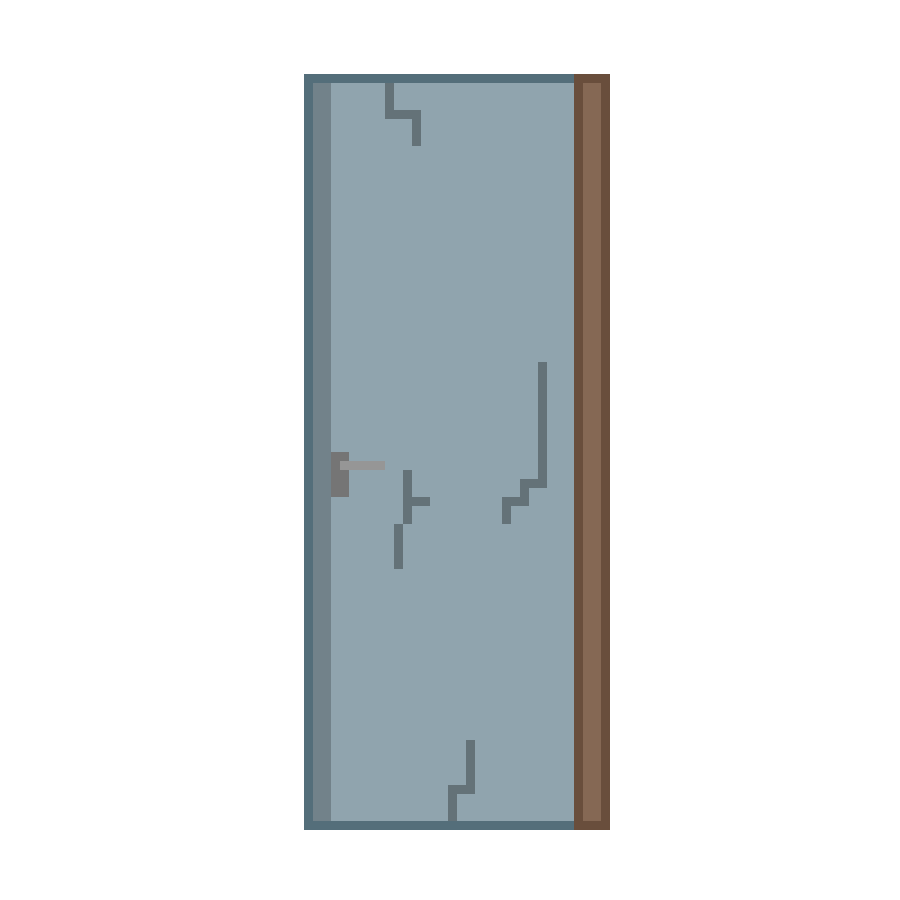
\includegraphics[width=1\linewidth]{figs/vidu/referencia_porta_tutorial (1).png}
        \caption{\small Sprite da porta C aberta}
        \label{fig:viduPortaC1}
    \end{subfigure}
    \begin{subfigure}{0.18\linewidth}
        \centering
        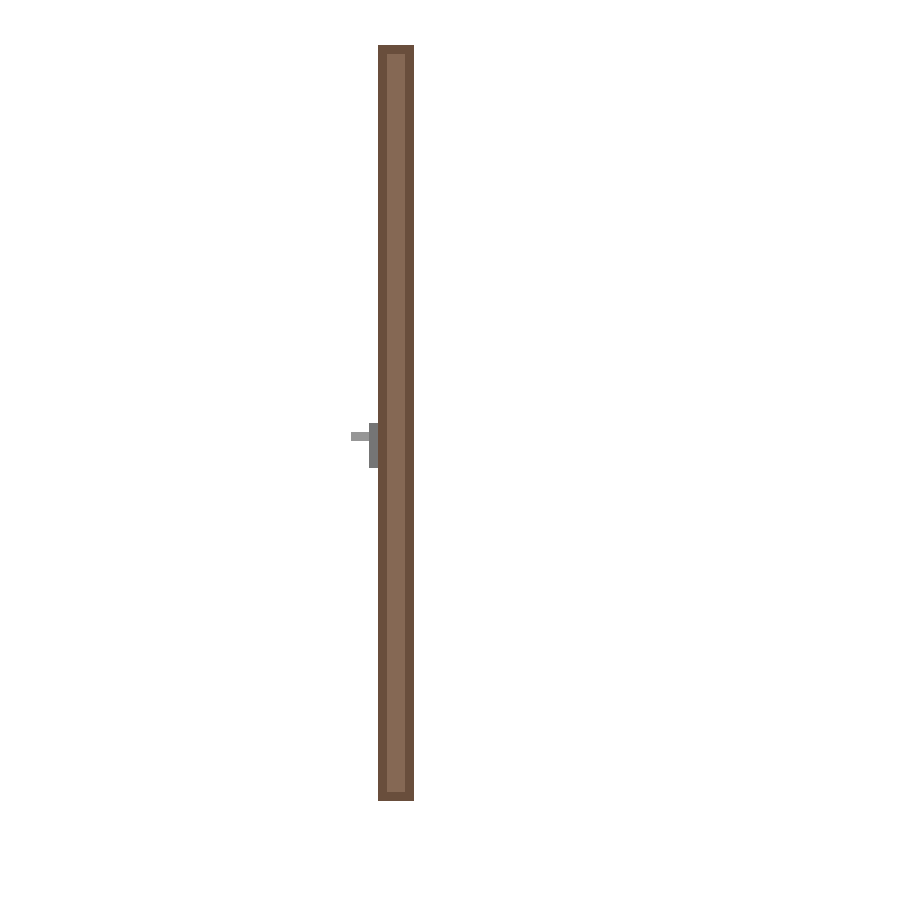
\includegraphics[width=1\linewidth]{figs/vidu/referencia_porta_tutorial (2).png}
        \caption{\small Sprite da porta C fechada}
        \label{fig:viduPortaC2}
    \end{subfigure}
    \begin{subfigure}{0.18\linewidth}
        \centering
        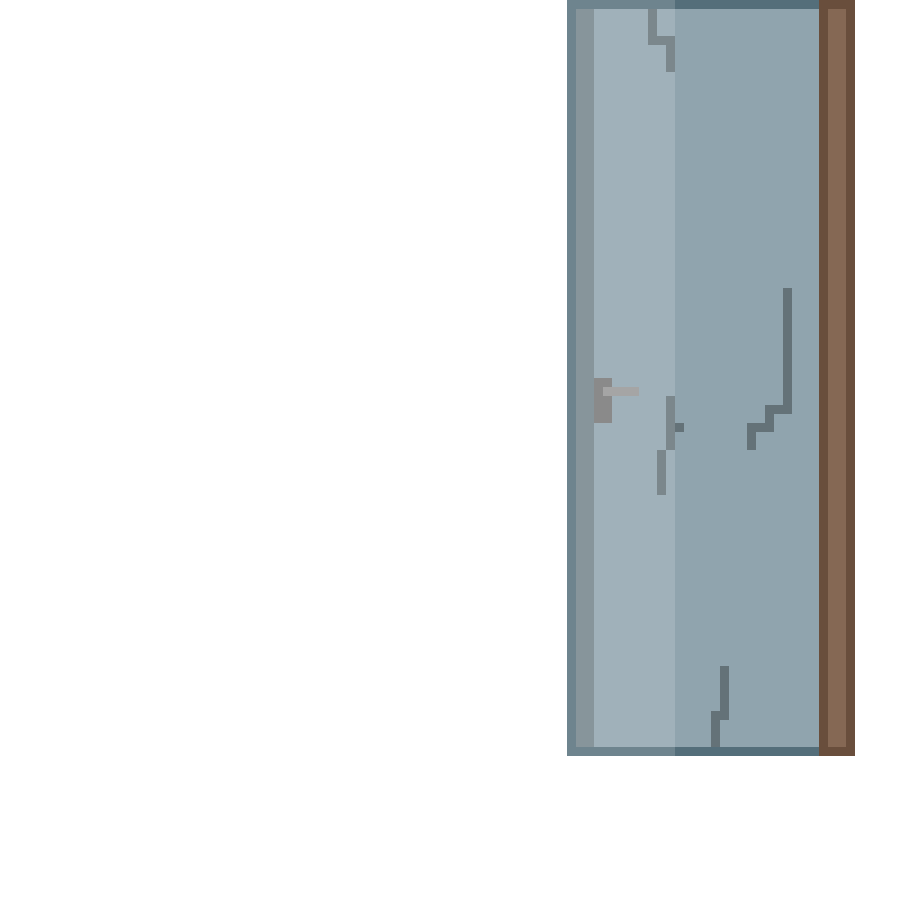
\includegraphics[width=1\linewidth]{figs/vidu/referencia_porta_tutorial (3).png}
        \caption{\small Sprite da porta C mais aberta}
        \label{fig:viduPortaC3}
    \end{subfigure}
    \begin{subfigure}{0.45\linewidth}
        \centering
        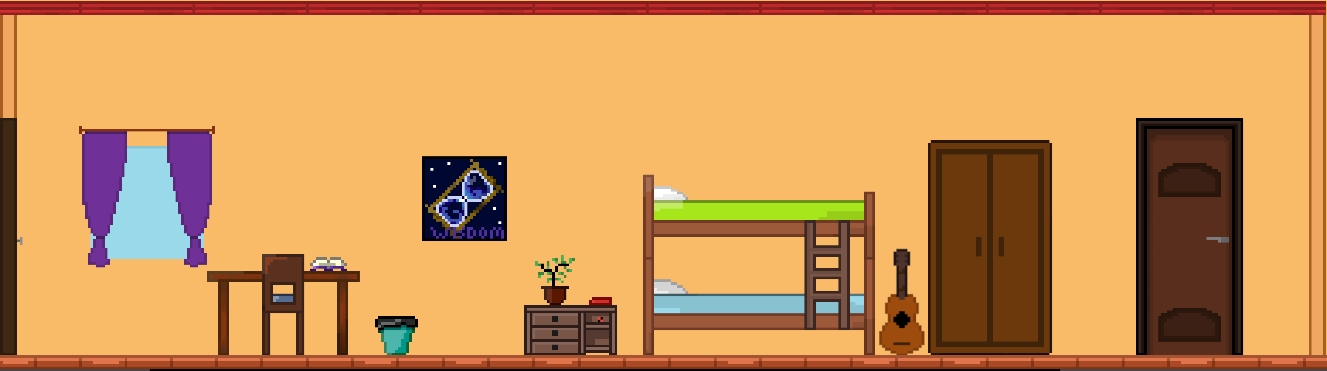
\includegraphics[width=1\linewidth]{figs/vidu/referencia_quarto.PNG}
        \caption{\small Referência do quarto do Pablo}
        \label{fig:viduQuartoPablo}
    \end{subfigure}
    \begin{subfigure}{0.45\linewidth}
        \centering
        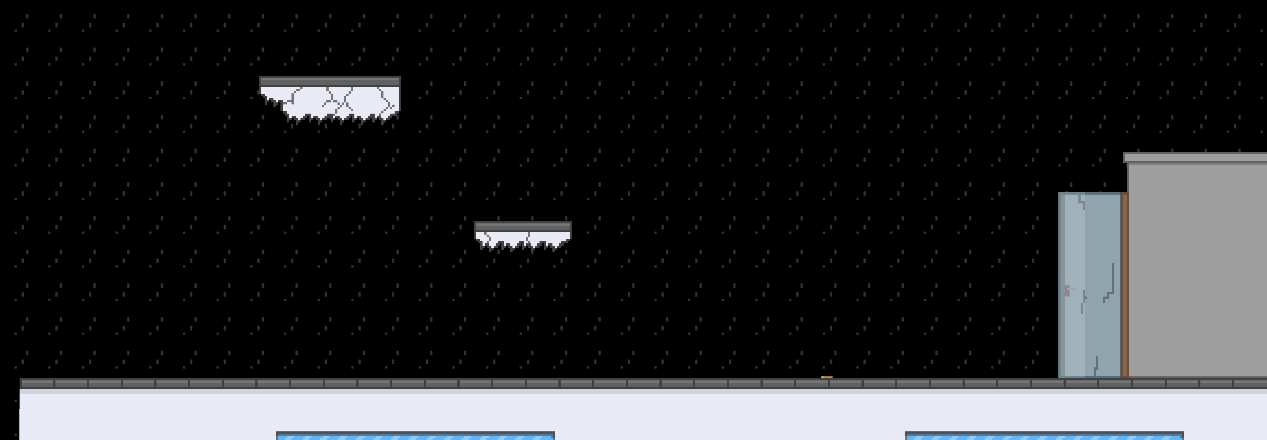
\includegraphics[width=1\linewidth]{figs/vidu/referencia_tutorial.PNG}
        \caption{\small Referência do tutorial}
        \label{fig:viduTutorial}
    \end{subfigure}
    \legend{\small Fonte: Elaborada pela autora.}
\end{figure}

%ver tudo que tentou criar
Durante a análise, o objetivo mudou de acordo com as necessidades do projeto, e alguns testes mais ambiciosos foram feitos. No total, foi tentado criar animações do personagem Pablo andando, pulando, abrindo a porta, se deitando/levantando da cama, e de diferentes portas abrindo.

%   ------------------------------------------------------------------------
\FloatBarrier
\subsection{Funcionalidade de referência para vídeo}
\label{s.vidu.referencia}


Os primeiros testes realizados, usando o sprite em front view (Figura \ref{fig:viduPablo}) para criação da animação de caminhada em side view, deixaram evidente uma grande dificuldade da ferramenta em manter o ambiente 2D, transformando o personagem para o 3D em um estilo cúbico, numa tentativa de replicar o estilo pixel art tridimensionalmente e mantendo as características físicas consistentes com a referência. Além disso, os resultados\footnote{\url{https://drive.google.com/drive/folders/10WGbLbvQspGPJlN8q57Up7GsKqN250aA?usp=drive_link}} adicionavam uma paisagem ao fundo e mostravam o personagem andando na diagonal, uma direção não presente no jogo desenvolvido. 

%fundo recorda o jogo minecraft

Porém, em um dos resultados, os erros de dimensão e direção foram corrigidos, formando uma animação 2D e realmente em side view. A Figura \ref{fig:viduComparaDimensao} apresenta a diferença entre os resultados, comparando um quadro do vídeo em 3D com um do em 2D.

\begin{figure}[htbp]
    \centering
    \caption{\small Comparação do resultado 3D e 2D gerado pelo Vidu}
    \label{fig:viduComparaDimensao}
    \begin{subfigure}{0.45\linewidth}
        \centering
        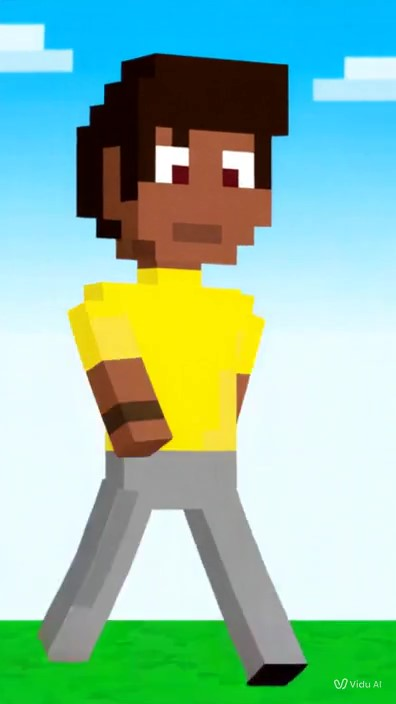
\includegraphics[width=0.8\linewidth]{figs/vidu/frame2.jpg}
        \caption{\small Frame da animação em 3D, com estilo cúbico e andando na diagonal}
        \label{fig:viduFrame3D}
    \end{subfigure}
    \begin{subfigure}{0.45\linewidth}
        \centering
        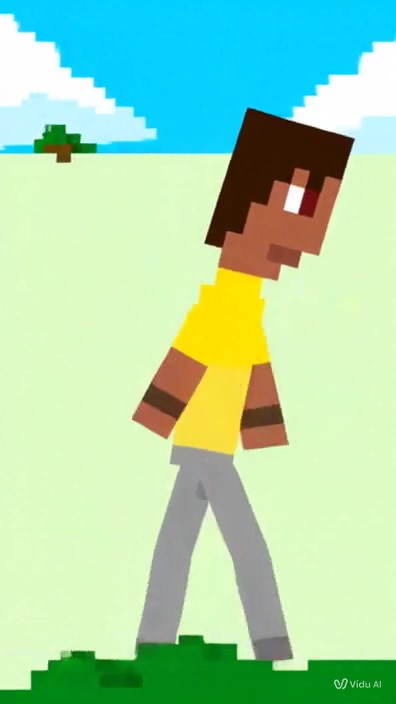
\includegraphics[width=0.8\linewidth]{figs/vidu/frame3.jpg}
        \caption{\small Frame da animação em 2D, andando em side view}
        \label{fig:viduFrame2D}
    \end{subfigure}
    \legend{\small Fonte: Elaborada pela autora, utilizando a ferramenta Vidu.}
\end{figure}

Apesar disso, a nova imagem formada para o personagem em side view possuía a cabeça muito quadrada e, mesmo que o design ainda fosse em pixel art, a animação deformava esse estilo, da mesma forma que aconteceu com a ferramenta Animated Drawnings (descrita na Seção \ref{s.sketchLab}). Outro detalhe observado nesse vídeo específico foi que, durante a animação de andar, o personagem nem sempre dobra a perna ou, quando dobra, é muito pouco, formando uma movimentação que causa estranheza ao olhar. A postura inclinada para frente, o movimento brusco do braço e a quantidade variável de movimentação do mesmo contribuem para esse estranhamento. 

Para entender a causa de apenas um dos testes produzir o vídeo em 2D, analisou-se a metodologia de cada um deles. A principal diferença encontrada foi a estrutura do prompt textual. Como a plataforma mostra de exemplo (Figura \ref{fig:viduPromptExemplo}), nos vídeos em 3D, a tag da imagem de referência foi usada como sujeito da frase (Figura \ref{fig:viduPrompt3d}). Enquanto no vídeo em 2D, a instrução foi mais imperativa e descritiva, sem considerar a tag como uma palavra a ser usada e apenas como forma de marcar que a imagem foi anexada (Figura \ref{fig:viduPrompt2D}). Baseado nisso, levanta-se a hipótese de que, ao não tratar a imagem como um sujeito imutável, a IA teve maior liberdade para reinterpretar o personagem e criar um novo sprite 2D em side view, em vez de apenas rotacionar a imagem de referência, o que mantinha características do sprite em front view e adicionava profundidade para parecer parcialmente de lado.

\begin{figure}[htbp]
    \centering
    \caption{\small Exemplo de prompt mostrado no Vidu}
    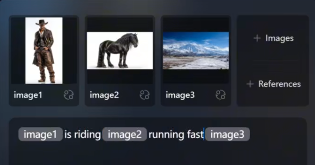
\includegraphics[width=0.6\linewidth]{figs/vidu/promptEx.PNG}
    \label{fig:viduPromptExemplo}
    \legend{\small Fonte: Elaborada pela autora.}
\end{figure}

\begin{figure}[htbp]
    \centering
    \begin{minipage}{0.45\textwidth}
    \centering
    \caption{\small Prompt que gerou vídeo em 3D no Vidu}
    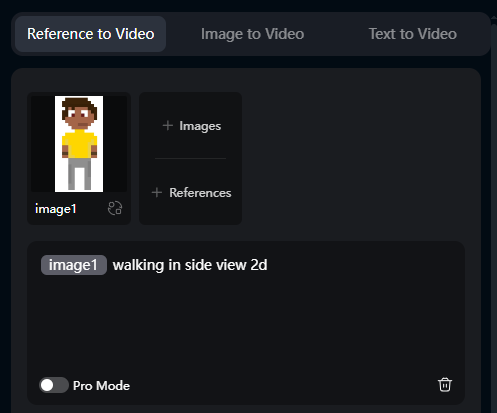
\includegraphics[width=0.9\linewidth]{figs/vidu/prompt2.PNG}
    \label{fig:viduPrompt3d}
    \legend{\small Fonte: Elaborada pela autora.}
    \end{minipage}\hfill
    \begin{minipage}{0.45\textwidth}
    \centering
    \caption{\small Prompt que gerou vídeo em 2D no Vidu}    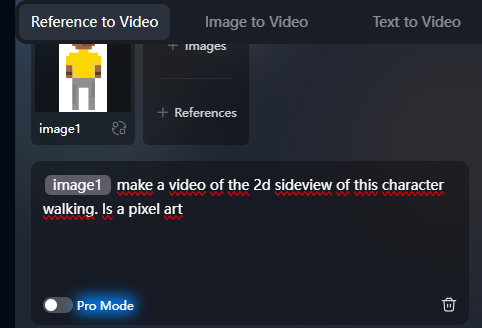
\includegraphics[width=0.9\linewidth]{figs/vidu/prompt3.PNG}
    \label{fig:viduPrompt2D}
    \legend{\small Fonte: Elaborada pela autora.}
    \end{minipage}\hfill
    
\end{figure}

Comparando tudo, foi notado que o vídeo em 2D aparentava possuir mais frames com partes borradas em relação às animações em 3D. Para confirmar essa teoria, os vídeos foram transformados em sprite sheet, com a ferramenta ezgif\footnote{https://ezgif.com/} (transforma vídeo em gif, e gif em sprite sheet), e foi feita uma análise quadro a quadro, verificando quais frames apresentavam uma grande deformação e nenhuma deformação.

\begin{table}[htbp]
    \centering
    \caption{Análise quantitativa de frames com deformação nos vídeos gerados pelo Vidu}
    \label{tab:viduDeformacoes}
    \begin{tabular}{l c c c}
        \toprule
        \textbf{Nível de deformação} & \textbf{Vídeo 1 (3D)} & \textbf{Vídeo 2 (3D)} & \textbf{Vídeo 3 (2D)} \\
        \midrule
        Deformação grave (\%) & 7,32\% & 12,2\% & \textbf{36,59\%} \\
        (Frames) & 3 &  5 & \textbf{15} \\
        \midrule
        Deformação leve (\%) & 48,78\%  & 41,46\% & 39,02\% \\
        (Frames)& 20 & 17 & 16 \\
        \midrule
        Sem deformação (\%) & 43,9\% & 46,34\% & \textbf{24,39\%} \\
        (Frames)&18 & 19 & \textbf{10}\\
        \midrule
        \textbf{Total (\%)} & 100\% & 100\% & 100\%  \\
        \textbf{(Frames)} & 41 & 41 & 41 \\
        \bottomrule
    \end{tabular}
    \legend{\small Fonte: Elaborada pela autora.}
\end{table}

A Tabela \ref{tab:viduDeformacoes} comprova a hipótese. O vídeo gerado em 2D, apresentou uma taxa de frames com deformação grave (partes muito borradas) quase duas vezes maior que a taxa somada dos vídeos em 3D. Consequentemente, o número de frames sem deformação foi quase metade em comparação com as versões 3D. As Figuras \ref{fig:viduNiveisDeformacao1} a \ref{fig:viduNiveisDeformacao3} apresentam exemplos visuais que definem cada categoria de deformação utilizada na análise de cada um dos vídeos.

\begin{figure}[htbp]
    \centering
    \caption{\small Quadros do Vídeo 1 (3D) em cada um dos níveis de deformação}
    \label{fig:viduNiveisDeformacao1}
    \begin{subfigure}{0.32\linewidth}
        \centering
        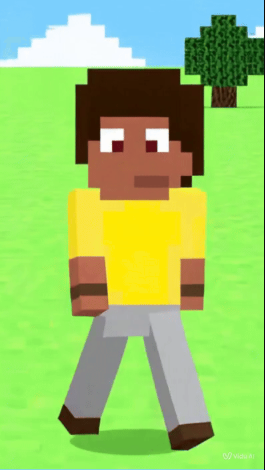
\includegraphics[width=0.8\linewidth]{figs/vidu/1sem.png}
        \caption{\small Quadro classificado como sem deformação}
        \label{fig:viduDeformacao1Sem}
    \end{subfigure}
    \begin{subfigure}{0.32\linewidth}
        \centering
        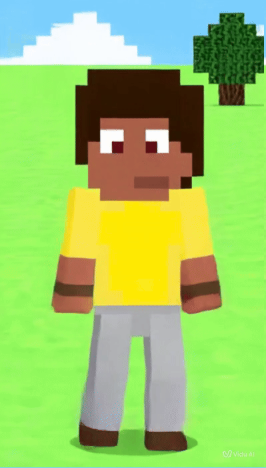
\includegraphics[width=0.8\linewidth]{figs/vidu/1leve.png}
        \caption{\small Quadro com deformação leve (borda da perna com pequenas ondulações)}
        \label{fig:viduDeformacao1Leve}
    \end{subfigure}
    \begin{subfigure}{0.32\linewidth}
        \centering
        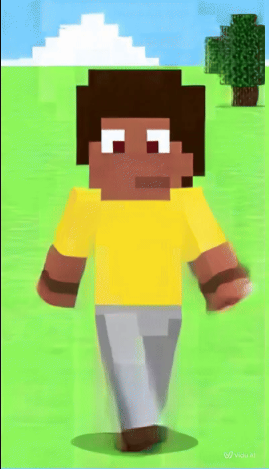
\includegraphics[width=0.8\linewidth]{figs/vidu/1grave.png}
        \caption{\small Quadro com deformação grave (perna e mão embaçados)}
        \label{fig:viduDeformacao1Grave}
    \end{subfigure}
    \legend{\small Fonte: Elaborada pela autora, utilizando a ferramenta Vidu.}
\end{figure}


\begin{figure}[htbp]
    \centering
    \caption{\small Quadros do Vídeo 2 (3D) em cada um dos níveis de deformação}
    \label{fig:viduNiveisDeformacao2}
    \begin{subfigure}{0.32\linewidth}
        \centering
        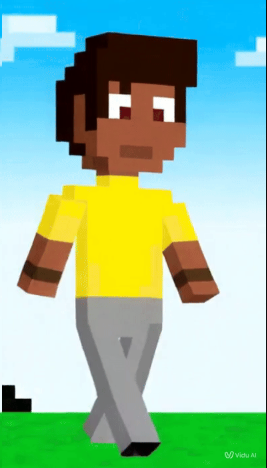
\includegraphics[width=0.9\linewidth]{figs/vidu/2sem.png}
        \caption{\small Quadro classificado como sem deformação}
        \label{fig:viduDeformacao2Sem}
    \end{subfigure}
    \begin{subfigure}{0.32\linewidth}
        \centering
        
\includegraphics[width=0.9\linewidth]{figs/vidu/2leve.png}
        \caption{\small Quadro com deformação leve (perna e bracelete levemente borrados)}
        \label{fig:viduDeformacao2Leve}
    \end{subfigure}
    \begin{subfigure}{0.32\linewidth}
        \centering
        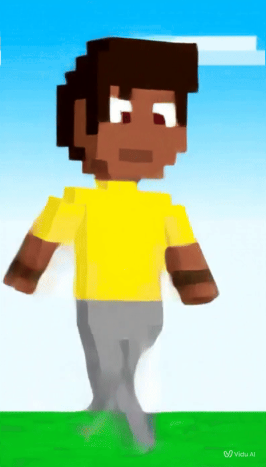
\includegraphics[width=0.9\linewidth]{figs/vidu/2grave.png}
        \caption{\small Quadro com deformação grave (perna deformada, olhos e braços levemente embaçados)}
        \label{fig:viduDeformacao2Grave}
    \end{subfigure}
    \legend{\small Fonte: Elaborada pela autora, utilizando a ferramenta Vidu.}
\end{figure}


\begin{figure}[htbp]
    \centering
    \caption{\small Quadros do Vídeo 3 (2D) em cada um dos níveis de deformação}
    \label{fig:viduNiveisDeformacao3}
    \begin{subfigure}{0.32\linewidth}
        \centering
        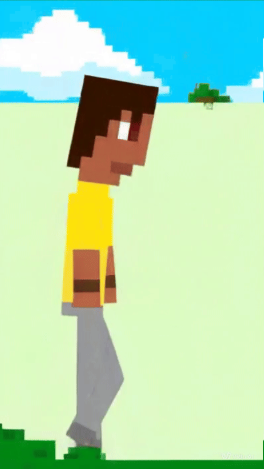
\includegraphics[width=1\linewidth]{figs/vidu/3sem.png}
        \caption{\small Quadro classificado como sem deformação}
        \label{fig:viduDeformacao3Sem}
    \end{subfigure}
    \begin{subfigure}{0.32\linewidth}
        \centering
        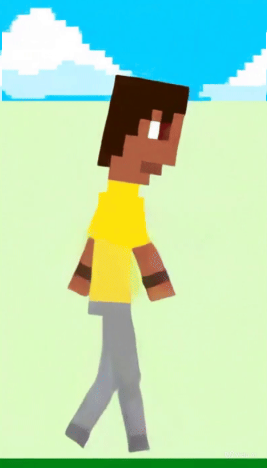
\includegraphics[width=1\linewidth]{figs/vidu/3leve.png}
        \caption{\small Quadro com deformação leve (borda da perna com pequenas ondulações )}
        \label{fig:viduDeformacao3Leve}
    \end{subfigure}
    \begin{subfigure}{0.32\linewidth}
        \centering
        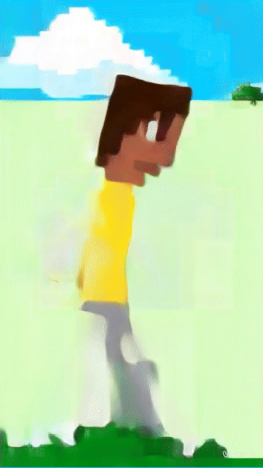
\includegraphics[width=1\linewidth]{figs/vidu/3grave.png}
        \caption{\small Quadro com deformação grave (rosto e corpo borrados, sem braços)}
        \label{fig:viduDeformacao3Grave}
    \end{subfigure}
    \legend{\small Fonte: Elaborada pela autora, utilizando a ferramenta Vidu.}
\end{figure}


O aumento de deformações no resultado 2D possui duas causas prováveis: ou a estrutura do prompt menos restritiva (sem usar a tag como sujeito) resultou em maior instabilidade, ou a ferramenta Vidu possui uma dificuldade em manter a qualidade quadro a quadro ao gerar animações 2D, sendo mais otimizada para a manipulação de referências em 3D.

A interação completa dessa primeira bateria de testes pode ser consultada na Figura \ref{fig:vidu1} no Apêndice \ref{ap.telasIA}.

Para tentar corrigir os erros encontrados nos vídeos, uma segunda bateria de testes foi realizada. Desta vez, foi utilizada como imagem de referência o melhor sprite em side view disponível até o momento (Figura \ref{fig:viduPabloChatGPTSide}). A expectativa era que, ao fornecer uma imagem já na perspectiva correta, a IA teria menos dificuldade em gerar uma animação 2D consistente, sem causar erro na direção e dimensão, além de apresentar um sprite mais adequado.

Os resultados\footnote{\url{https://drive.google.com/drive/folders/1oUOF8-v87bZVZkrv7cTRFy0qcgdaMPZL?usp=sharing}} confirmaram parcialmente a expectativa, eliminando em maior parte o problema da geração em 3D. Entretanto, eles introduziram novos erros. A movimentação do personagem tornou-se ainda mais imprecisa, com a IA adicionando novas ações como pular e girar (Figura \ref{fig:viduGirar}), e fazendo o personagem sair da tela (Figura \ref{fig:viduSair}). Ao modificar a proporção da geração de vídeo, com o objetivo do personagem ter mais espaço para se movimentar sem sair do enquadramento, o sprite passou a deslizar horizontalmente de maneira imprevisível. Ademais, em um dos casos, de forma contraintuitiva, adicionar a palavra 2D ao prompt resultou em uma animação 2D que se tornava 3D ao final (Figura \ref{fig:vidu2D3D}). 


\begin{figure}[htbp]
    \centering
    \begin{minipage}{0.45\textwidth}
    \centering
    \caption{\small Frame do personagem girando para outra direção}
    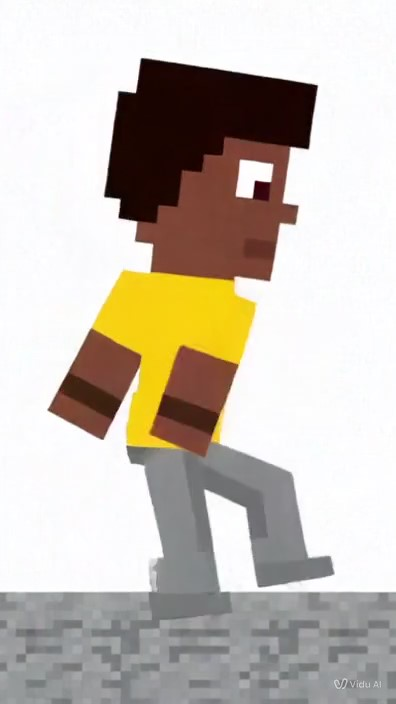
\includegraphics[width=0.6\linewidth]{figs/vidu/frameGirar.jpg}
    \label{fig:viduGirar}
    \legend{\small Fonte: Elaborada pela autora, utilizando a ferramenta Vidu.}
    \end{minipage}\hfill
    \begin{minipage}{0.45\textwidth}
    \centering
    \caption{\small Frame do personagem saindo da tela}    
    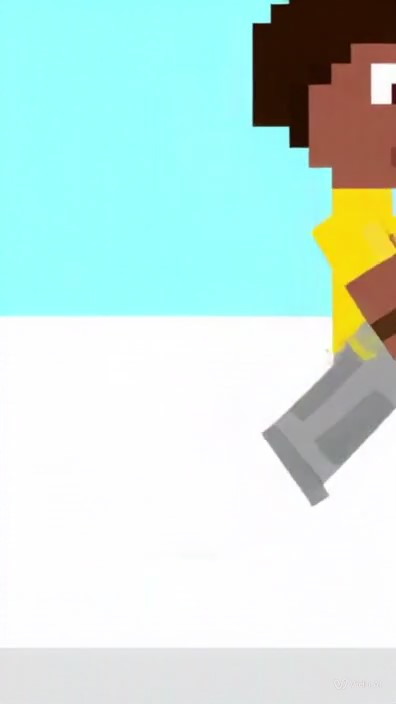
\includegraphics[width=0.6\linewidth]{figs/vidu/frameSairTela.jpg}
    \label{fig:viduSair}
    \legend{\small Fonte: Elaborada pela autora, utilizando a ferramenta Vidu.}
    \end{minipage}\hfill
\end{figure}

\begin{figure}[htbp]
    \centering
    \caption{\small Frame do vídeo gerado em 3D após adicionar a palavra 2D no prompt no Vidu}
    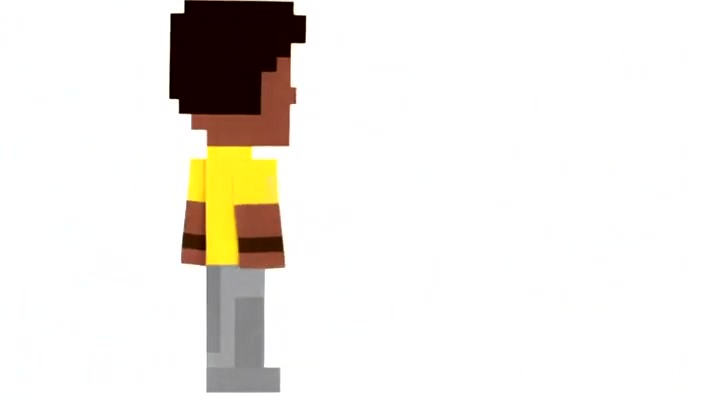
\includegraphics[width=0.5\linewidth]{figs/vidu/frame5_3D.jpg}
    \label{fig:vidu2D3D}
    \legend{\small Fonte: Elaborada pela autora, utilizando a ferramenta Vidu.}
\end{figure}\hfill

Nessa segunda bateria de testes, foi possível gerar um resultado em 2D utilizando a tag da imagem como sujeito do prompt. Mesmo assim, a animação ainda apresentou a inconsistência no movimento, o que indica que a estrutura anterior de prompt não foi a causa dessa instabilidade.

Numa tentativa de corrigir um dos erros que se manteve em praticamente todos os resultados nessa ferramenta, a presença de uma paisagem ao fundo que dificulta o processo de extrair apenas a animação, foi solicitado um vídeo com fundo transparente (utilizando a tag da imagem como sujeito). O resultado gerado foi uma animação 3D, que manteve o movimento de andar na direção incorreta.

A interação completa pode ser consultada nas Figuras \ref{fig:vidu2} a \ref{fig:vidu5} no Apêndice \ref{ap.telasIA}.

Para aprofundar a análise e confirmar a hipótese sobre a dificuldade da ferramenta com o 2D, a mesma análise quantitativa de deformação nos quadros foi replicada nos novos vídeos. 

\begin{table}[htbp]
    \centering
    \caption{Análise quantitativa de frames com deformação, comparando testes com referência em front e side view.}
    \label{tab:viduDeformacoesCompleta}
    \resizebox{\textwidth}{!}{% Redimensiona a tabela para caber na largura da página
    \begin{tabular}{l c c | c c c c c}
        \toprule
        & \multicolumn{2}{c|}{\textbf{Front View como referência}} & \multicolumn{5}{c}{\textbf{Side View como referência}} \\
        \textbf{Nível de deformação} & \textbf{Vídeo 2 (3D)} & \textbf{Vídeo 3 (2D)} & \textbf{Vídeo 1a (2D)} & \textbf{Vídeo 1b (2D)} & \textbf{Vídeo 2 (2D/3D)} & \textbf{Vídeo 3 (2D)} & \textbf{Vídeo 4 (3D)} \\
        \midrule
        Deformação grave (\%) & \textbf{12,2}\% & 36,6\% & 17,1\% & 22,0\% & 26,8\% & 48,8\textbf{\%} & \textbf{12,2}\% \\
        (Frames) & \textbf{5} & 15 & 7 & 9 & 11 & 20 & \textbf{5} \\
        \midrule
        Deformação leve (\%) & 41,5\% & 39,0\% & 56,1\% & 63,4\% & 56,1\% & 34,1\% & 48,8\% \\
        (Frames) & 17 & 16 & 23 & 26 & 23 & 14 & 20 \\
        \midrule
        Sem deformação (\%) & \textbf{46,3\%} & 24,4\% & 26,8\% & 14,6\% & 17,1\% & 17,1\% & \textbf{39,0\%} \\
        (Frames) & \textbf{19} & 10 & 11 & 6 & 7 & 7 & \textbf{16} \\
        \bottomrule
    \end{tabular}
    }
    \legend{\small Fonte: Elaborada pela autora.}
\end{table}

A Tabela \ref{tab:viduDeformacoesCompleta} apresenta os dados de ambas as baterias de testes, permitindo uma comparação direta e reforçando a hipótese de que as deformações são decorrentes da dificuldade da ferramenta com a geração de uma animação 2D, não tendo relação direta com a maneira em que o prompt é estruturado. Primeiramente, observa-se que todos os vídeos gerados em 2D, independentemente da imagem de referência e da estrutura de prompt, apresentam uma taxa de deformação grave e um número de frames sem deformação significativamente piores do que qualquer um dos vídeos gerados em 3D. Embora o uso de uma referência em side view tenha melhorado a estabilidade em alguns casos (Vídeo 1a na Tabela \ref{tab:viduDeformacoesCompleta}), a qualidade geral permaneceu baixa e outros erros sempre estavam presentes.

Outro fator observado foi que no vídeo 2 da segunda bateria de testes, dos 11 frames com deformação grave, apenas 2 deles eram em 3D. Enquanto isso, dos 7 frames sem deformação, 5 deles eram em 3D. Isso mostra que até mesmo durante o mesmo vídeo, a qualidade melhorou no momento em que a animação se tornou 3D.

Crucialmente, como já foi comentado, nesta segunda bateria de testes foi possível gerar um resultado em 2D (nomeado como Vídeo 3 na Tabela \ref{tab:viduDeformacoesCompleta}) utilizando a tag da imagem como sujeito. O fato de a animação ainda assim apresentar a maior taxa de deformação de todos os testes (48,8\%) invalida a hipótese de que a estrutura do prompt era a causa principal da falha. A evidência agora aponta de forma mais conclusiva para a segunda hipótese: a ferramenta Vidu possui uma dificuldade em manter a consistência e a qualidade ao gerar animações em 2D.


Após as análises anteriores revelarem as dificuldades do Vidu na geração de animações 2D, o foco dos testes foi redefinido, explorando a capacidade da ferramenta em usar mais de uma imagem para a geração do vídeo. Tendo em vista que uma animação de caminhada satisfatória já havia sido obtida com a ferramenta Gemini Pro (detalhada na Seção \ref{s.ferramentaB}), o objetivo dos próximos testes no Vidu passou a ser a geração de animações com interações entre personagens, objetos e lugares. 

%outras ferramentas que possuíam uma limitação de apenas uma imagem

Além disso, uma exploração mais aprofundada da funcionalidade de referência para vídeo revelou uma forma distinta de utilização da mesma: em vez de anexar uma imagem para ser considerada como referência, a plataforma permite criar uma referência nomeada. Essa opção permite associar um nome a um conjunto de imagens de diferentes ângulos e a uma descrição, com a hipótese de que, ao fornecer à IA uma compreensão mais completa do personagem, a consistência da animação gerada poderia ser melhorada.

Primeiro, foram criadas as referências do personagem Pablo (Figuras \ref{fig:viduPablo},\ref{fig:viduPabloGeminiProSide} e \ref{fig:viduPabloGeminiProBack}), do beliche (Figura \ref{fig:viduCama}), da porta marrom (Figuras \ref{fig:viduPortaA} e \ref{fig:viduPortaB}), da porta cinza (Figuras \ref{fig:viduPortaC1} a \ref{fig:viduPortaC3}), do quarto do Pablo (Figura \ref{fig:viduQuartoPablo}) e da cena do tutorial (Figura \ref{fig:viduTutorial}). Essa criação possuía duas etapas:
\begin{itemize}
    \item Anexar imagens que representam a referência e escolhendo um nome para ela (Figura \ref{fig:viduReferenciaPablo1}); e
    \item Revisar o estilo e a descrição da referência, geradas automaticamente (Figura \ref{fig:viduReferenciaPablo2}).
\end{itemize}

\begin{figure}
    \centering
    \caption{\small Tela da primeira etapa da criação de referência do personagem Pablo no Vidu}
    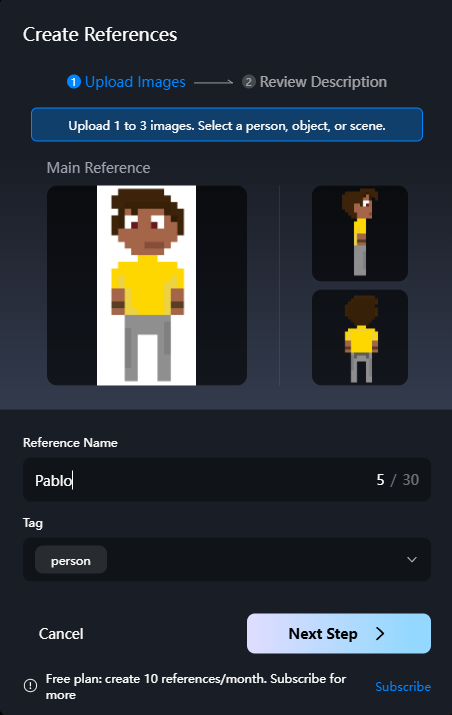
\includegraphics[width=0.3\linewidth]{figs/vidu/tela_referencia.PNG}
    \label{fig:viduReferenciaPablo1}
    \legend{\small Fonte: Elaborada pela autora.}

\end{figure}

\begin{figure}[htbp]
    \centering
    \caption{\small Tela da segunda etapa da criação de referência do personagem Pablo no Vidu}
    \label{fig:viduReferenciaPablo2}
    \begin{subfigure}{0.4\linewidth}
        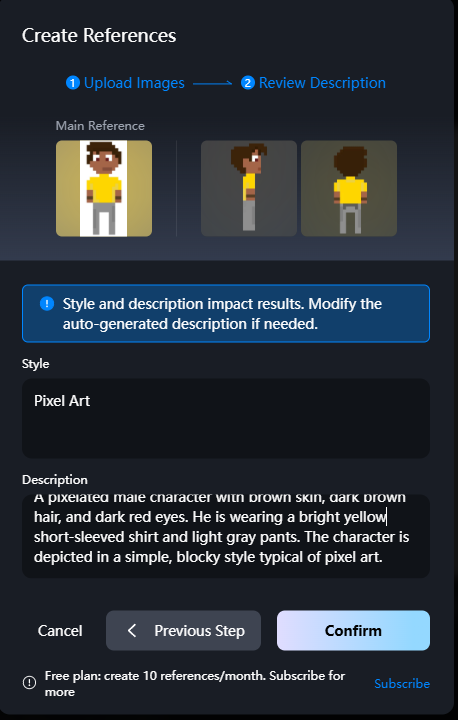
\includegraphics[width=1\linewidth]{figs/vidu/tela_referencia_2.PNG}
        \caption{\small Descrição e estilo gerados automaticamente pela IA}
        \label{fig:viduReferenciaPablo2a}
    \end{subfigure}
    \begin{subfigure}{0.4\linewidth}
        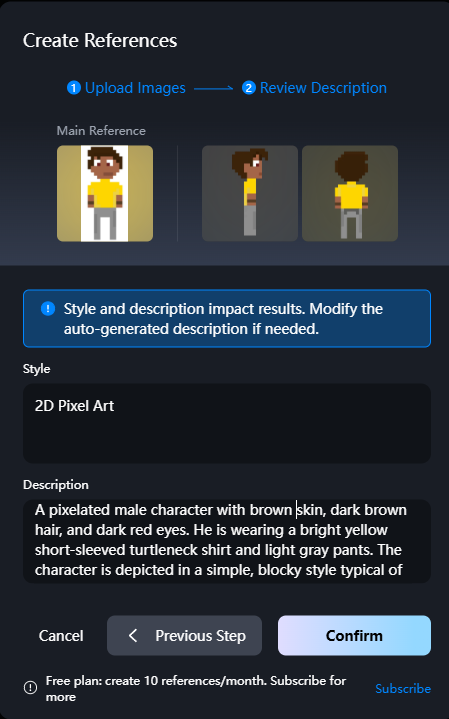
\includegraphics[width=1\linewidth]{figs/vidu/tela_referencia_2_editado.PNG}
        \caption{\small Estilo e descrição revisado manualmente, adicionando a palavra 2D no estilo e especificando o tipo de camisa na descrição}
        \label{fig:viduReferenciaPablo2b}
    \end{subfigure}
    \legend{\small Fonte: Elaborada pela autora.}
\end{figure}

As referências restantes criadas podem ser conferidas nas Figuras \ref{fig:viduReferenciaCama} a \ref{fig:viduReferenciaTutorial} no Apêndice \ref{ap.telasIA}.

Inicialmente, nessa nova bateria de testes, o objetivo era criar uma animação do personagem deitado se levantando da cama. Para isso, o nome das referências substituiu o que seria a descrição do personagem e do objeto. O resultado\footnote{\url{https://drive.google.com/file/d/1LG15atEW7Eba102-ADYkqW0z4RIYG67O/view?usp=sharing}} parecia promissor, mantendo boa parte das características do personagem e da cama, mantendo um cenário 2D e o estilo correto. Porém, ao analisar melhor o vídeo, é possível notar imprecisões no design do personagem e do beliche. O beliche gerada sofre um grande nível de zoom, cortando parte do sprite, além de que a cama debaixo possui dois travesseiros (um de cada lado) e a escada foi distorcida e movida para a lateral da cama de cima (Figura \ref{fig:viduErrosCama}). O personagem possuía características de ângulos diferentes em momentos errados, como a sua calça que ficou igual à do sprite em back view mesmo quando o personagem estava virado para frente ou para o lado (Figura \ref{fig:viduErrosPablo}). Além disso, a IA fez o personagem inicialmente sentado na cama, em vez de deitado, e apresentou frames borrados. 

\begin{figure}[htbp]
    \centering
    \caption{\small Inconsistências do beliche circuladas, em vermelho o segundo travesseiro e em azul a escada distorcida}
    \label{fig:viduErrosCama}
    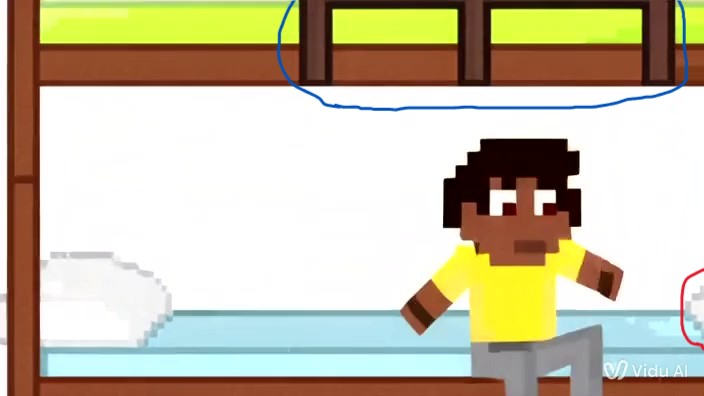
\includegraphics[width=0.7\linewidth]{figs/vidu/errosCama.jpg}
    \legend{\small Fonte: Elaborada pela autora.}
\end{figure}

\begin{figure}[htbp]
    \centering
    \caption{\small Inconsistência do personagem circulado}
    \label{fig:viduErrosPablo}
    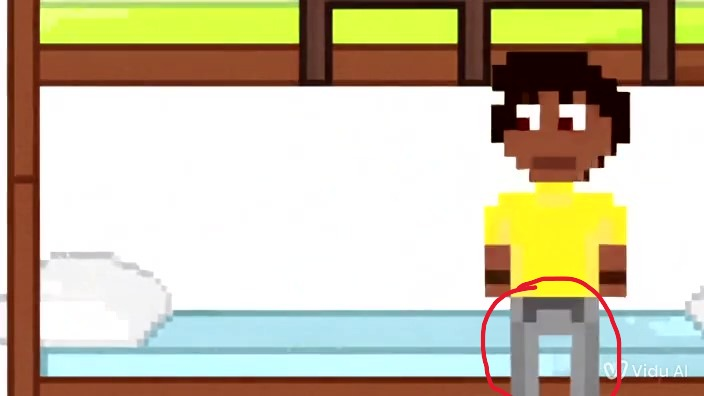
\includegraphics[width=0.7\linewidth]{figs/vidu/errosPablo.JPG}
    \legend{\small Fonte: Elaborada pela autora.}
\end{figure}

Para tentar criar a animação com o personagem realmente se levantando após estar deitado, foi feito um novo prompt especificando que o Pablo devia se deitar e, após isso, se levantar. O resultado\footnote{\url{https://drive.google.com/file/d/1PHQvJ2kcFuv2NWMyS08FiMOpw8_T9ygG/view?usp=sharing}} foi bem pior que o esperado. Apesar do personagem ter ficado mais consistente, a cama ficou muito mais incongruente, além da ação solicitada não ser gerada. O beliche foi dividida em partes e remontada como se fossem duas camas, a verde tendo virado metade verde e metade azul com dois travesseiros (Figura \ref{fig:viduErrosCama2}).

\begin{figure}[htbp]
    \centering
    \caption{\small Beliche fragmentado}
    \label{fig:viduErrosCama2}
    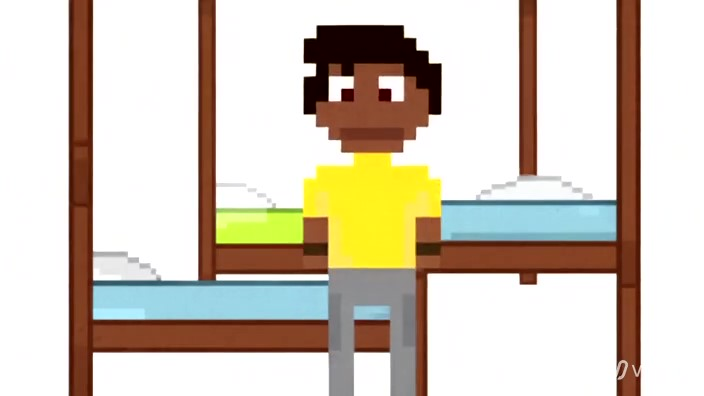
\includegraphics[width=0.7\linewidth]{figs/vidu/frame7.jpg}
    \legend{\small Fonte: Elaborada pela autora, utilizando a ferramenta Vidu.}
\end{figure}

Numa tentativa de gerar uma animação com o beliche mais consistente, foi também usado o quarto para ser o cenário da animação. A hipótese era que a falta de um fundo definido pudesse estar fazendo com que a IA modificasse a cama para ficar menos vazio o ambiente. O resultado\footnote{\url{https://drive.google.com/file/d/1PLl_ThD7HTMA2iA1j4OQ3exOZDhML5ZJ/view?usp=sharing}} gerou o personagem deitado e se levantando, porém as incongruências do beliche foram mantidas. Além disso, o quarto também não era idêntico à referência (apesar das características serem as mesmas, a forma com que elas eram desenhadas não era igual) e o personagem se teleportava de um lado para o outro na cama antes de sair dela. Esses detalhes podem ser verificados na Figura \ref{fig:viduVideoQuarto}.

%O beliche estava conectada ao beliche já existente no cenário do quarto como devia ser, mas deformou mesmo assim

\begin{figure}[htbp]
    \centering
    \caption{\small Quadro do vídeo gerado no Vidu}
    \label{fig:viduVideoQuarto}
    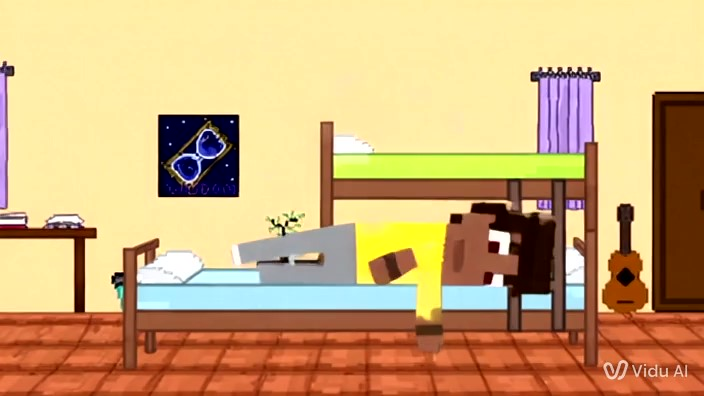
\includegraphics[width=0.7\linewidth]{figs/vidu/frame8.jpg}
    \legend{\small Fonte: Elaborada pela autora, utilizando a ferramenta Vidu.}
\end{figure}

%REVISAR SE EU CONSEGUIR IMPLEMENTAR A ANIMAÇÃO NO JOGO E MODIFICAR ELA

Em uma última tentativa utilizando apenas o personagem e a cama, o resultado\footnote{\url{https://drive.google.com/file/d/1caNcLrZhx69wZk3ShfJYDh1qzkkP57Zo/view?usp=sharing}} apresentou uma melhora significativa. Embora ainda apresentasse inconsistências, como uma leve mudança de perspectiva da cama e o personagem deslizando antes de iniciar o movimento, a estrutura do beliche foi gerada com maior precisão, e a ação principal de levantar-se foi executada.

Apesar de ter sido a melhor animação produzida pela ferramenta até o momento, o resultado ainda exigiria um processo de edição manual extenso para ser considerado satisfatório, incluindo a potencial remoção do beliche para ajustar a animação do personagem diretamente no cenário do jogo. Considerando que o esforço de modificação seria desproporcional à importância desta animação para o projeto, optou-se por não editar ou implementar o resultado final.

Na bateria de testes seguinte, o objetivo foi produzir uma animação do personagem abrindo a porta. Por causa dos erros de consistência do personagem nos vídeos anteriores, foi adicionada na descrição do Pablo uma parte especificando o ângulo de cada imagem (Figura \ref{fig:viduReferenciaPabloEditado} do Apêndice \ref{ap.telasIA}). 

Os resultados\footnote{\url{https://drive.google.com/drive/folders/1aWPXy7SAJmMUJlEvNTxy2__ntK6ZjZy6?usp=drive_link}} apresentaram ou deformações na porta (Figura \ref{fig:viduPortaChao}) ou imprecisões na animação da abertura dela (Figura \ref{fig:viduPortaAbrindo}). Apesar do movimento em específico do personagem ser adequado, é possível encontrar quadros onde ele possui incongruências (Figura \ref{fig:viduDoisBraceletes}) e a alta taxa de frames deformados ainda continua. A interação completa pode ser consultada nas Figuras \ref{fig:vidu10} a \ref{fig:vidu12} do Apêndice \ref{ap.telasIA}.

% sem fundo = distorce porta
%descrição fundo ou quarto fundo = porta consistente


\begin{figure}[htbp]
    \centering
    \caption{\small Porta deformada para fazer o chão no vídeo gerado pelo Vidu}
    \label{fig:viduPortaChao}
    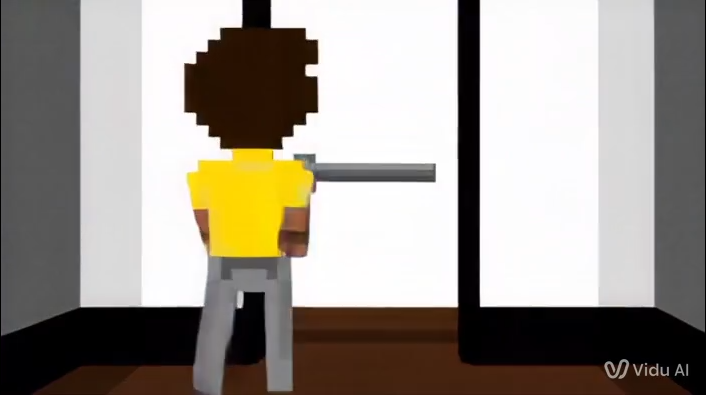
\includegraphics[width=0.6\linewidth]{figs/vidu/porta_deformada.PNG}
    \legend{\small Fonte: Elaborada pela autora, utilizando a ferramenta Vidu.}
\end{figure}

\begin{figure}[htbp]
    \centering
    \caption{\small Porta abrindo pelo lado errado no vídeo gerado pelo Vidu}
    \label{fig:viduPortaAbrindo}
    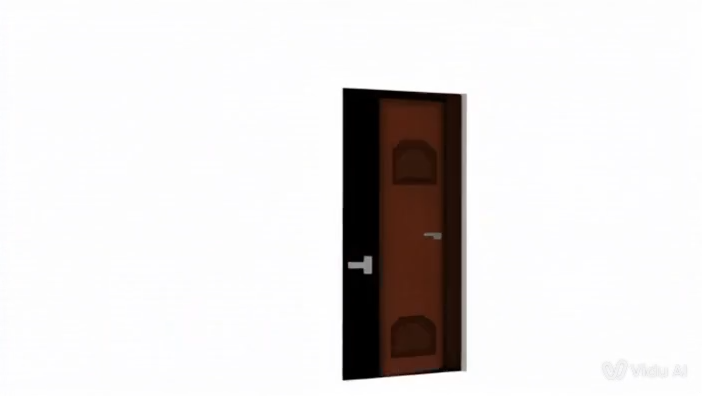
\includegraphics[width=0.7\linewidth]{figs/vidu/porta_abrindo_lado_oposto.PNG}
    \legend{\small Fonte: Elaborada pela autora, utilizando a ferramenta Vidu.}
\end{figure}

\begin{figure}[htbp]
    \centering
    \caption{\small Dois braceletes no braço do personagem no vídeo gerado pelo Vidu}
    \label{fig:viduDoisBraceletes}
    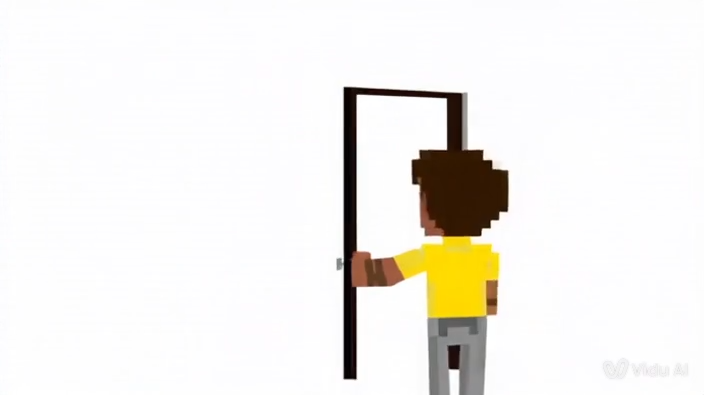
\includegraphics[width=0.7\linewidth]{figs/vidu/Braceletes.PNG}
    \legend{\small Fonte: Elaborada pela autora, utilizando a ferramenta Vidu.}
\end{figure}

Comparando as baterias de testes, notou-se que foi gerada a mesma área parcial do cenário nos testes em que o quarto foi utilizado, mesmo que a referência tivesse mais partes. Além disso, o beliche foi desenhado no mesmo lugar onde estava localizado no quarto, enquanto a porta foi posicionada numa região completamente distinta. 

Com a análise comparativa foi criada uma hipótese sobre o comportamento da IA: ela parece processar apenas a área central da imagem de referência do cenário. Como a beliche estava posicionada perto do centro da imagem do quarto, sua localização no vídeo foi correta. A porta, no entanto, que estava na borda da imagem de referência, foi cortada de sua posição original e gerada incorretamente no centro da cena.


\begin{figure}[htbp]
    \centering
    \caption{\small Comparação da geração dos objetos em relação ao quarto no Vidu}
    \label{fig:viduComparaLugar}
    \begin{subfigure}{0.4\linewidth}
        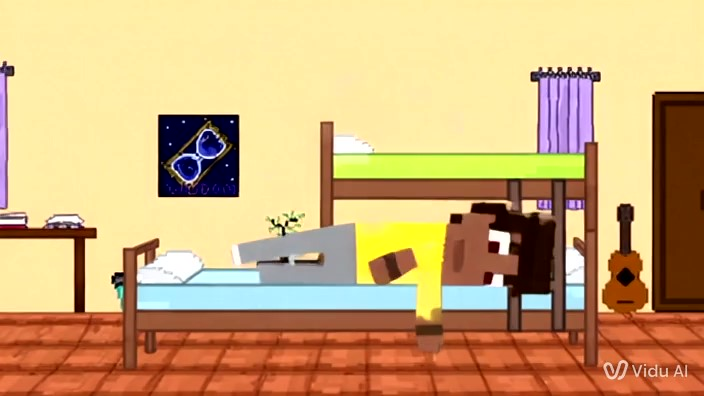
\includegraphics[width=1\linewidth]{figs/vidu/frame8.jpg}
        \caption{\small Beliche inconsistente posicionada no lugar correto}
        \label{fig:viduComparaBeliche}
    \end{subfigure}
    \begin{subfigure}{0.4\linewidth}
        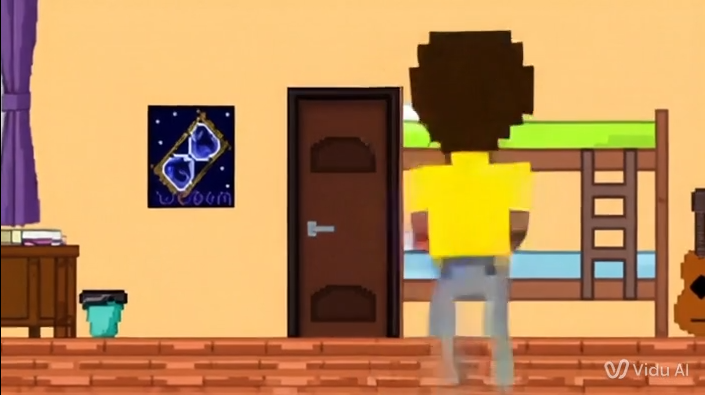
\includegraphics[width=1\linewidth]{figs/vidu/frame11.PNG}
        \caption{\small Porta consistente posicionada no lugar incorreto}
        \label{fig:viduComparaPorta}
    \end{subfigure}
    \legend{\small Fonte: Elaborada pela autora.}
\end{figure}

Em busca de tentar aprimorar os resultados, foi encontrada uma técnica mais complexa de criar prompts para a ferramenta do Vidu. Para gerar vídeos mais consistentes e unificados, foi necessário: destacar o estilo artístico, usar termos precisos e simples, descrever o sujeito, a cena e o ambiente, e utilizar palavras-chave atmosféricas \cite{docs_2025}. Dessa forma, um novo prompt foi idealizado (Figura \ref{fig:vidu13} do Apêndice \ref{ap.telasIA}), gerando um vídeo\footnote{\url{https://drive.google.com/file/d/1o_BNadSvUQ5w4TaJZ5DBUaw0V66rc-na/view?usp=sharing}} melhor que os anteriores. Os sprites não possuem inconsistência notável em relação à referência e a porta abre de maneira precisa, porém o personagem só segura a maçaneta após a porta abrir, além de que ela começou aberta e depois repentinamente tornou-se fechada. A animação da porta abrindo foi satisfatória, mesmo que o movimento do personagem para abri-la não tenha sido. Apesar disso, outra ferramenta foi capaz de gerar uma animação da mesma qualidade para a porta e com menos necessidade de edições porque o personagem não estava cobrindo parte do objeto.

Ainda usando essa nova estratégia de prompt, no próximo teste o objetivo passou a ser produzir uma animação do personagem pulando. Para isso foi utilizada apenas a imagem em side view em vez da referência Pablo, com o objetivo de evitar erros em que o personagem vira o corpo em outro ângulo no meio da animação. Os vídeos\footnote{\url{https://drive.google.com/drive/folders/1Lpi7zzY0BvaPkgjSv7xvc5aVubXCEVor?usp=drive_link}} criados não alcançaram as expectativas, renderizando um fundo branco e preto e fazendo com que o personagem parecesse estar caindo ou apenas pulando de um pé só. Além disso, essa animação específica demonstra uma grande taxa de quadros borrados, ainda maior do que o esperado. Interação pode ser consultada na Figura \ref{fig:viduPulo1} no Apêndice \ref{ap.telasIA}.

Também tentou-se criar uma animação para a porta abrindo, só que dessa vez em side view e sem a presença do personagem. Os resultados\footnote{\url{https://drive.google.com/drive/folders/1oplBZG15V_LfexCUw-X973PXb3gNfzIP?usp=drive_link}} não foram suficientes, sem produzir o movimento da porta abrir na visão correta, girando-a e até mesmo duplicando-a. Processo demonstrado nas Figuras \ref{fig:viduPorta1} e \ref{fig:viduPorta2}.

Em geral, essa funcionalidade da ferramenta apresentou grande potencial, porém possui uma grande queda de qualidade para gerar animações especificamente 2D, além de apresentar alguns erros de consistência e precisão. Esse método consegue fornecer uma base para a animação ser modificada manualmente, corrigindo diversos detalhes.


%   ------------------------------------------------------------------------
\FloatBarrier
\subsection{Funcionalidade de imagem para vídeo}
\label{s.vidu.imagem}

A funcionalidade de imagem para vídeo permite que o usuário defina o primeiro e, opcionalmente, o último frame do vídeo a ser gerado, além da clássica descrição do prompt, podendo especificar ações para diferentes quadros. 

Nos testes iniciais, o objetivo era criar uma animação das portas fechando ou abrindo (que ainda não havia sido feita na época). Nessa funcionalidade, não foi possível mais usar as referências criadas anteriormente, sendo possível apenas anexar uma imagem simples para os frames inicial e final. Utilizando as recomendações descobertas anteriormente, um prompt foi confeccionado para ser usado em todas as tentativas, que foi apenas levemente modificado de acordo com as necessidades.

Para a porta cinza, foi colocado o sprite dela aberta (Figura \ref{fig:viduPortaC3}) para o primeiro quadro, e a figura dela fechada (Figura \ref{fig:viduPortaC2}) para o último quadro. O resultado gerado\footnote{\url{https://drive.google.com/file/d/1MExWoA7CkPSTmd0MBEr3Z3-u9n4KmTfW/view?usp=sharing}} foi um sucesso parcial. A câmera se mexe de acordo com o movimento da porta, que foi distorcida a ponto de perder os detalhes das rachaduras e expandida na horizontal(Figura \ref{fig:viduPortaMaior}) antes de se fechar. Apesar disso, encontrou-se uma oportunidade de usar a animação como base para alguns ajustes, como adicionar as rachaduras novamente e manter a câmera fixa no mesmo ponto. Isso ocorreu pois o movimento de fechar foi feito mesmo que apenas após uma distorção do objeto (que pode ser cortada), e o estilo de pixel art foi mantido. %se nenhuma outra animação melhor for feita

\begin{figure}[htbp]
    \centering
    \caption{\small Quadro da porta expandindo na animação gerada no Vidu}
    \label{fig:viduPortaMaior}
    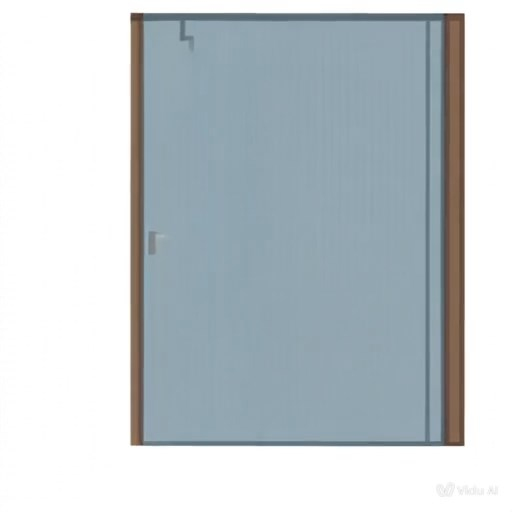
\includegraphics[width=0.4\linewidth]{figs/vidu/framePortaHorizontalMaior.jpg}
    \legend{\small Fonte: Elaborada pela autora, utilizando a ferramenta Vidu.}
\end{figure}

Para a porta marrom, apenas foi anexado ao quadro inicial o sprite dela aberta. Os resultados\footnote{\url{https://drive.google.com/drive/folders/1EOloiSlzuRKM0gus7U78opbw4Q6lfjr-?usp=sharing}} não foram satisfatórios. No primeiro vídeo, a porta abre pelo lado direito (oposto ao correto) como uma sanfona (Figura \ref{fig:viduPortaSanfona}), com o sprite da porta ao lado dele mesmo mais escuro, ambos inclinados formando uma ponta. Por causa disso, o prompt foi ajustado para especificar que a porta deveria abrir para o lado esquerdo. Mesmo assim, o resultado não foi preciso. A porta continuou abrindo do lado errado, além de desconectar-se da moldura no começo da animação (Figura \ref{fig:viduPortaDesconexao}). Uma melhora em relação à animação anterior foi que o frame final gerou a porta aberta quase sem nenhuma inconsistência (Figura \ref{fig:viduPortaAberta}). O processo completo para geração das animações das portas pode ser consultado nas Figuras \ref{fig:vidu14} e \ref{fig:vidu15} no Apêndice \ref{ap.telasIA}.

\begin{figure}[htbp]
    \centering
    \begin{minipage}{0.32\textwidth}
    \centering
    \caption{\small Quadro da porta parecendo uma sanfona}
    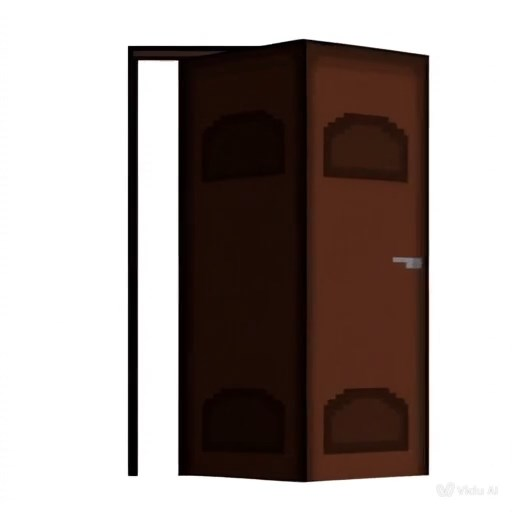
\includegraphics[width=1\linewidth]{figs/vidu/framePortaSanfona.jpg}
    \label{fig:viduPortaSanfona}
    \legend{\small Fonte: Elaborada pela autora, utilizando a ferramenta Vidu.}
    \end{minipage}\hfill
    \begin{minipage}{0.32\textwidth}
    \centering
    \caption{\small Quadro da porta desconectando da moldura}    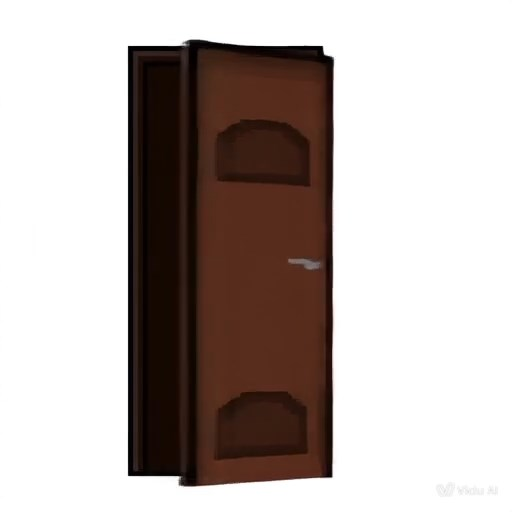
\includegraphics[width=1\linewidth]{figs/vidu/framePortaDesconexao.jpg}
    \label{fig:viduPortaDesconexao}
    \legend{\small Fonte: Elaborada pela autora, utilizando a ferramenta Vidu.}
    \end{minipage}\hfill
    \begin{minipage}{0.32\textwidth}
    \centering
    \caption{\small Quadro da porta aberta gerado no Vidu}    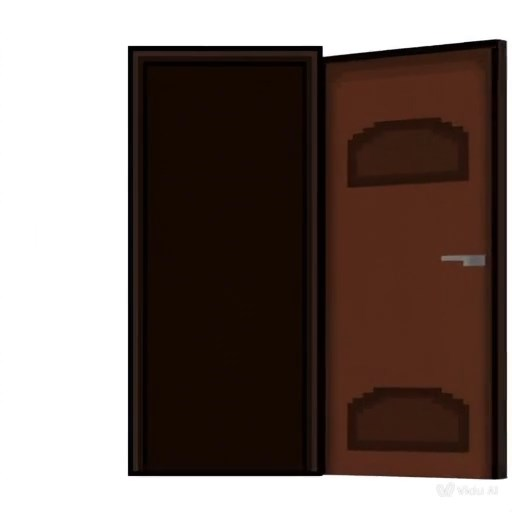
\includegraphics[width=1\linewidth]{figs/vidu/framePortaAberta.jpg}
    \label{fig:viduPortaAberta}
    \legend{\small Fonte: Elaborada pela autora, utilizando a ferramenta Vidu.}
    \end{minipage}\hfill
\end{figure}

No teste seguinte, o objetivo foi gerar uma animação para o pulo do personagem, visto que foi encontrada uma animação adequada para a porta marrom. O resultado\footnote{\url{https://drive.google.com/file/d/1QcPnZp21dFyTtQ_J57pV7zzT_W0MR8Js/view?usp=sharing}} foi extremamente insatisfatório, sem o movimento do pulo sequer ser gerado. No vídeo, o personagem dobra as pernas sem realmente se agachar e abre os braços, se inclinando para frente enquanto o fundo fica metade preto e os quadros ficam borrados (Figura \ref{fig:viduPuloInclina}).

\begin{figure}[htbp]
    \centering
    \caption{\small Quadro do personagem inclinando para frente na animação gerada no Vidu}
    \label{fig:viduPuloInclina}
    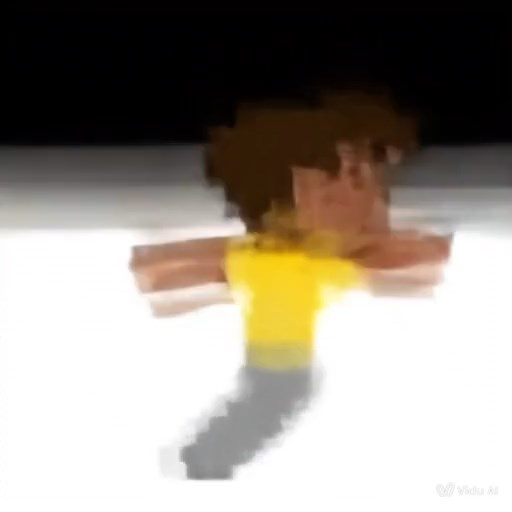
\includegraphics[width=0.4\linewidth]{figs/vidu/framePulo2.jpg}
    \legend{\small Fonte: Elaborada pela autora, utilizando a ferramenta Vidu.}
\end{figure}

A hipótese elaborada para a animação ter sido completamente imprecisa e com mudanças extras foi que, sem o frame final, a IA tem mais dificuldade em fazer movimentos onde a cena não acaba diferente do quadro inicial. O pulo não é um movimento linear: o personagem chega a um ponto mais alto e depois cai até a mesma altura em que se estava antes. Porém, a funcionalidade parece ter sido feita para mostrar uma progressão na transformação, chegar de um estado A para B sem nenhum terceiro ponto no caminho. Dessa forma, em busca de gerar uma mudança que gerasse uma progressão, foi modificado o fundo com o personagem apenas inclinando-se para frente em vez de fazer o movimento de ir para cima e depois para baixo.


Após algumas pesquisas mais aprofundadas na ferramenta, foi descoberto que os prompts para essa funcionalidade específica não funcionavam da mesma maneira que os do resto da ferramenta. É recomendado utilizar prompts curtos e visuais, mencionando o movimento da câmera e o estilo visual \cite{docs2_2025}. As sugestões foram feitas especificamente para o modelo Vidu Q1, porém, como citado anteriormente, o teste foi realizado no modelo Vidu 2.0.

Assim, durante o último teste, com o objetivo de gerar a animação da porta marrom em side view abrindo, é utilizado um prompt seguindo esse padrão. O resultado\footnote{\url{https://drive.google.com/file/d/1NfyI0P6tybE1VX_NeIegRJdKDVumBqmA/view?usp=sharing}} foi satisfatório, porém ele teria que passar por alguns ajustes antes de poder ser aplicado no jogo. A animação fez o movimento da porta abrindo, porém sem mover a maçaneta de lugar, como pode ser visto na Figura \ref{fig:viduPortaFinalAberta}.

\begin{figure}[htbp]
    \centering
    \caption{\small Porta em side view aberta na animação gerada no Vidu}
    \label{fig:viduPortaFinalAberta}
    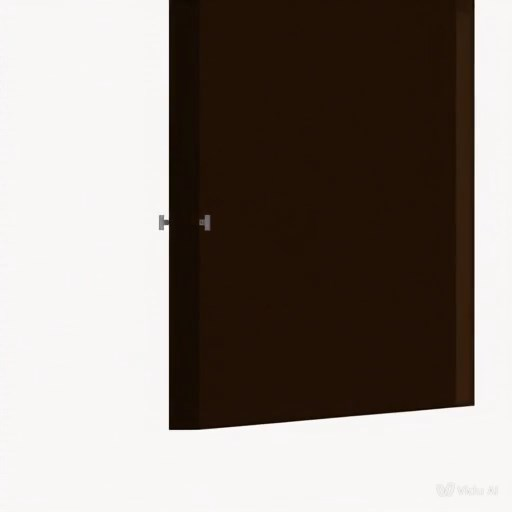
\includegraphics[width=0.4\linewidth]{figs/vidu/frameFinal.jpg}
    \legend{\small Fonte: Elaborada pela autora, utilizando a ferramenta Vidu.}
\end{figure}

Após o vídeo ter sido baixado, foi extraído seu sprite sheet pelo site ezgif (mencionado anteriormente) para ser possível fazer os ajustes com mais facilidade. Após isso, foi aberta a imagem no Pixilart (também mencionado anteriormente), transformando-a em uma verdadeira pixel art (Figura \ref{fig:viduPortaFinalSpriteSheetPixel}) onde seu fundo foi removido. Após isso, a animação estava pronta para ser exportada para a ferramenta Pixel Lab, onde foi realizado o pós-processamento (detalhado na Seção \ref{s.pixelLab}).

\begin{figure}[htbp]
    \centering
    \caption{\small Sprite sheet em pixel sem fundo da animação da porta em side view abrindo}
    \label{fig:viduPortaFinalSpriteSheetPixel}
    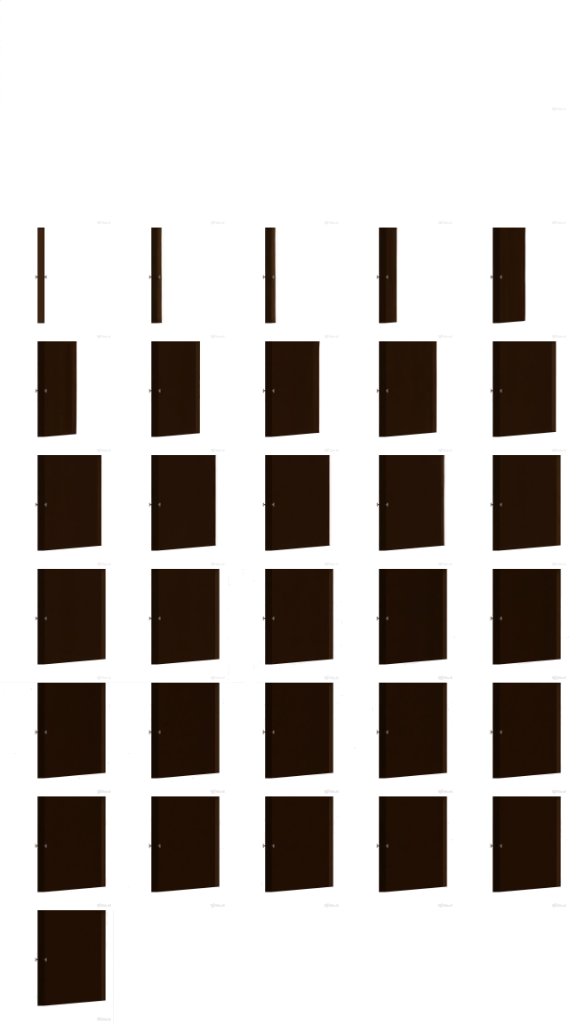
\includegraphics[width=0.4\linewidth]{figs/vidu/Pixilart/porta_sprite_sheet_pixel.png}
    \legend{\small Fonte: Elaborada pela autora, utilizando a ferramenta Pixilart.}
\end{figure}

Conclui-se que essa funcionalidade específica, ao trabalhar com frames definidos, suaviza a dificuldade da ferramenta em manter a consistência em 2D, observada na análise anterior. As falhas apresentadas foram relacionadas à imprecisão da interpretação do prompt e a uma aparente limitação com movimento de progressão não linear, como o pulo. A ferramenta demonstrou grande potencial e consistência para gerar um movimento fluído entre quadros-chave já desenhados, produzindo resultados que, embora precisem de ajustes finos, tornam o processo de animação mais eficiente.



